%%%%%%%%%%%%%%%%%%%%%%%%% file draft4_2.tex %%%%%%%%%%%%%%%%%%%%%%%%%%%%%%%
%	                                                                   %
% Based on the  template file for The European Physical Journal C          %
%                                                                          %
%                                                                          %
%                                                                          %
%                                                                          % 
%%%%%%%%%%%%%%%%%%%%%%%%% Springer-Verlag %%%%%%%%%%%%%%%%%%%%%%%%%%%%%%%%%%

\documentclass[epj,nopacs]{svjour}
\usepackage{graphics}
\usepackage{epsfig}
\usepackage{latexsym}
\usepackage{amssymb}
\usepackage[utf8]{inputenc}
\usepackage{../../assets/uniinput}

\usepackage{siunitx}
\usepackage[justification=raggedright,singlelinecheck=false]{caption}
\sisetup{
	seperr		=	true,
	trapambigerr	=	true,
	openerr		=	(,
	closeerr	=	),
	expproduct	=	cdot,
	padnumber	=	both,
	stickyper	=	true,
	per		=	slash,
	trapambigfrac	=	true,
	repeatunits	=	false,
	openfrac	=	(,
	closefrac	=	),
	prefixsymbolic 	=	true,
	prefixproduct	=	cdot,
	decimalsymbol	=	.,
        tabnumalign     =       left,
        tabtextalign    =       left
}

\newcommand{\spar}{{\stackrel{\rightarrow}{\Rightarrow}}}
\newcommand{\sant}{{\stackrel{\rightarrow}{\Leftarrow}}}
\newcommand{\sperpa}{{\rightarrow\Uparrow}}
\newcommand{\sperpb}{{\rightarrow\Downarrow}}

\setlength{\marginparwidth}{1cm}
\usepackage[textsize=tiny,colorinlistoftodos]{todonotes}

\hyphenation{calo-rimeter}

\begin{document}
\hugehead

\newcommand{\dd}[1]{\mathrm{d}#1\,} % declare dx operator, usage: \dd{x} for dx
\newcommand{\lref}[1]{listing~(\ref{lst:#1})} % refer to a listing, usage:\lref{label} for Listing (...)
\newcommand{\fref}[1]{fig.~(\ref{fig:#1})} % refer to a figure, usage:\lref{label} for Abb. (...)
\newcommand{\tref}[1]{tab.~(\ref{tab:#1})} % refer to a table, usage:tlref{label} for Tab. (...)
\newcommand{\eref}[1]{eq.~(\ref{eqn:#1})} % refer to a equation, usage:\eref{label} for Gl. (...)

\title{Z-Resonance at LEP}
\titlerunning{Z-Resonance at LEP}
\authorrunning{Thomas Murach, Robert Riemann}
\author{{\bf Draft Version 1.1}\\
\medskip \\
Thomas Murach,$^{1}$
Robert Riemann$^{1}$
} 
\institute{$^1$Department of Physics, Humboldt University of Berlin, Germany\\}  
\date{Received: \today / Revised version: 0.1}
\abstract{
This paper describes the analysis of the L3 detector data taken at different
center of mass energies around \SI{90}{\GeV}, which reveals the properties of
the $Z$-Boson. Additionally the weak mixing angle and the colour factor are determined.
The Z-boson mass is evaluated to $M_Z = \SI{91.16(3)}{\GeV}$ with a decay width
of $Γ_Z = \SI{2.61(6)}{\GeV}$.
The weak mixing angle is computed to $\sin² Θ_W = \num{0.23(9)}$ and the colour
factor to $N_C = \num{3.2(13)}$.
All resuls are in good agreement with the prediction and can be considered
as one of its best confirmations.
}

\maketitle

%%%%%%%%%%%%%%%%%%%%%%%%%%%%%%%%%%%%%%%%%%%%%%%%%%%%%%%%%%%%%%%%%%%%%%%%%%%%%%
\vspace*{-1.5cm}
\section{ Introduction}
\baselineskip=0.38cm
\vspace*{1.cm}

The standard model of elementary particles describes interactions of particles
by four fundamental forces. Two of them, the electric and the weak forces, can
be seen as one force, the electroweak force. Its gauge
bosons, which mediate the force between the two interacting particles, are the
photon as well as the $W^{\pm}$- and the $Z^0$-boson. The $Z^0$, which has been
discovered first at ..., could be produced extensively at the
electron-positron-collider LEP at CERN , which was possible
because of the sufficient center of mass energy of this collider experiment.

We were able to evaluate its mass $M_Z$ and its lifetime τ. The leptonic and
the hadronic decay widths $Γ_l$ and $Γ_{\mathrm{had}}$ could be investigated as
well. Finally
the number of quark colours $N_C$ and the weak mixing angle, also
called Weinstein angle, $\Theta_W$ can be measured. This angle describes the
ratio of the electromagnetic and the weak coupling constants α and α$_w$.

\section{ Experimental setup}

LEP was designed to be able to deliver center of mass energies $\sqrt{s}$ from
some 89 up to \SI{209}{\giga\electronvolt}. This is enough to produce Z-bosons,
which has a mass of about \SI{91}{\giga\electronvolt}, as it was
known from former measurements at SPPS. Therefore the Z$^0$-particle was
supposed to be produced at LEP.

It can decay in various ways, but always into pairs of one
fermion and one antifermion. One of these possibilities is the decay via two
different quarks (Z$^0→qq'$), another one could be the decay via two
charged leptons like Z$^0→ μ^+μ^-$. The first one of the mentioned decays can be
seen as two jets which can be measured in hadronic calorimeters. The leptonic
decay is measured due to registration of leptons in electromagnetic
calorimeters and muon chambers. All of the mentioned
detector layers have an almost cylindrical shape in order to
cover as much of the solid angle as possible. This is also the reason for the
installation of the end caps.

The particle detector LEP is built in a way as can be seen in \fref{aufbau}.
\begin{figure}[htb]
 \centering
 \includegraphics[page=5,viewport=286 620 508 765,clip,%
  width=\columnwidth,keepaspectratio]{../../Z0/docs/Z0ResFprakt}
 \caption{Design of the L3 detector \cite{pic}.}
%  \todo[inline]{soll hier eine quelle hin?}
 \label{fig:aufbau}
\end{figure}
There are layers of components with different purposes. Starting from the
interaction point, these are the tracking chamber, the electromagnetic
calorimeter, the hadronic calorimeter and finally the muon chamber.

In this case the hadronic calorimeter and the muon chamber are the most
important parts, because in this study we focuss on muonic and hadronic
Z$^0$-decays. The hadronic calorimeter consists of alternating layers of
uranium plates and wire chambers. The muon chamber is built up of drift
chambers. It detects the high energy muons, which have passed the detector
without a significant loss of energy, because these are the only particles that
are able to reach there.
% Further information about the detector design can be found in \cite{script}.

\section{ Data analysis}

For a detailed analysis of the mentioned processes it is important to be able
to distinguish between muonic and hadronic decays. By Monte Carlo studies the
differences between both processes could be figured out using pure hadronic and
muonic data samples as well as simulated data.
% , which was necessary
% because the hadronic and muonic cross sections and decay widths are going to
% be calculated seperately.
This facilitates the
possibility to apply cuts on the measured distributions.

In this paper first results of measurements at center of mass energies of
\num{89.48}, \num{91.33} and \SI{93.02}{\giga\electronvolt} will be presented.

\subsection{ Event selection}
Muons barely interact with any matter, therefore there are only very few
entries in the calorimeter along the track of the muon. This has an immense
discriminating power, because jets consist of tens of particles due to
hadronization at high energies and the decay of unstable particles inside the
jets.

Due to inefficiencies in energy measurement it is possible that not all the
energy provided by the apparatus can finally be seen. Therefore there are large
uncertainties in jet energy measurements, whereas these uncertainties are
smaller for muonic events. Nevertheless also for these events there is a
statistical uncertainty limiting the energetic resolution. This fact can also be
used to distinguish these
events from each other and from background as well. For example if the $Z^0$
decays into two very unstable tauons, these tauons decay very fast. Then two
neutrinos are created, but they cannot be measured, so that their contribution
to the visible energy is missing. The visible part of the tau decays resembles
hadronic events, so it is important to be able to separate this background from
the hadronic signal.

To be able to separate muonic events from background it is suitable to ask for
an angle of almost π between the two muons, as the $Z^0$ boson should be created
almost resting in
the laboratory frame, leading to muons flying back to back. Another selection
for muonic events is possible through the requirement of both muons carrying
about half the energy of the event each. This is possible because muon energies
can be measured very well. Finally it is possible to recognize muons through
their mass.

\subsection{Hadronic events}
As it is now known how to extract hadronic events out of the data, it is
possible to determine the hadronic cross section using the following formula:
\begin{equation}
σ_{\mathrm{had}} = \frac{N}{Lε},
\label{eqn:sigma}
\end{equation}
where ε is the efficiency of the cuts. The acceptance can be interpreted as an
additional factor set to 1, which is included in the efficiency. This efficiency
could be calculated using the following equation:
\begin{equation}
ε = \frac{N’_{\mathrm{MC}}}{N_{\mathrm{MC}}},
\end{equation}
where $N’_{\mathrm{MC}}$ is the number of Monte Carlo events that passed the
hadron cuts and $N_{\mathrm{MC}}$ is the total number of events in the Monte
Carlo file.

The hadronic cross section could be calculated at three different center of
mass energies. The number of hadronic events that passed the hadron cuts can be
found in \tref{hadr_events}, as well as the hadronic cross sections themselves.

\begin{table}[h]
\begin{center}
\begin{tabular}{|l|l|l|}
\hline
energy $\sqrt{s}$ [\si{\GeV}] & hadronic events & cross section
$σ^{\mathrm{had}}$ [\si{\nano\barn}]\\
\hline
89.48 & 1848 ± 43 ± 52 & 10.55 ± 0.18 ± 0.16 \\
91.33 & 3980 ± 63 ± 79 & 29.98 ± 0.49 ± 0.43 \\
93.02 & 2149 ± 46 ± 51 & 14.56 ± 0.24 ± 0.24 \\
\hline
\end{tabular}
\vspace*{0.3cm}
\caption{\baselineskip=0.38cm analyzed hadronic events at different center of
mass energies. The first given error is the statistical, the second one is the
systematic uncertainty.}
\label{tab:hadr_events}
\end{center}
\vspace*{-0.5cm}
\end{table}

The systematic uncertainties listed in this table are derived from the
systematic uncertainties of $ε_{\mathrm{had}}$ and the influence of variations
of the cuts.

% These cross sections have then been used as data for a fit (see \fref{fit_hadrons}).
The listed cross sections have been used then to fit the Breit-Wigner distribution as
seen in \fref{fit_hadrons}. Additionally there is a second graph shown, which
is derived by the Breit-Wigner fit, but takes account for QCD effects like
initial and final state radiation.

By fitting the data
points the overall hadronic cross section $σ_0^{\mathrm{had}}$, the mass $M_Z$
and the decay width $Γ_Z$ of the $Z^0$-boson could be determined. The results
can be found in \tref{results}.

\begin{figure}[htb]
 \centering
 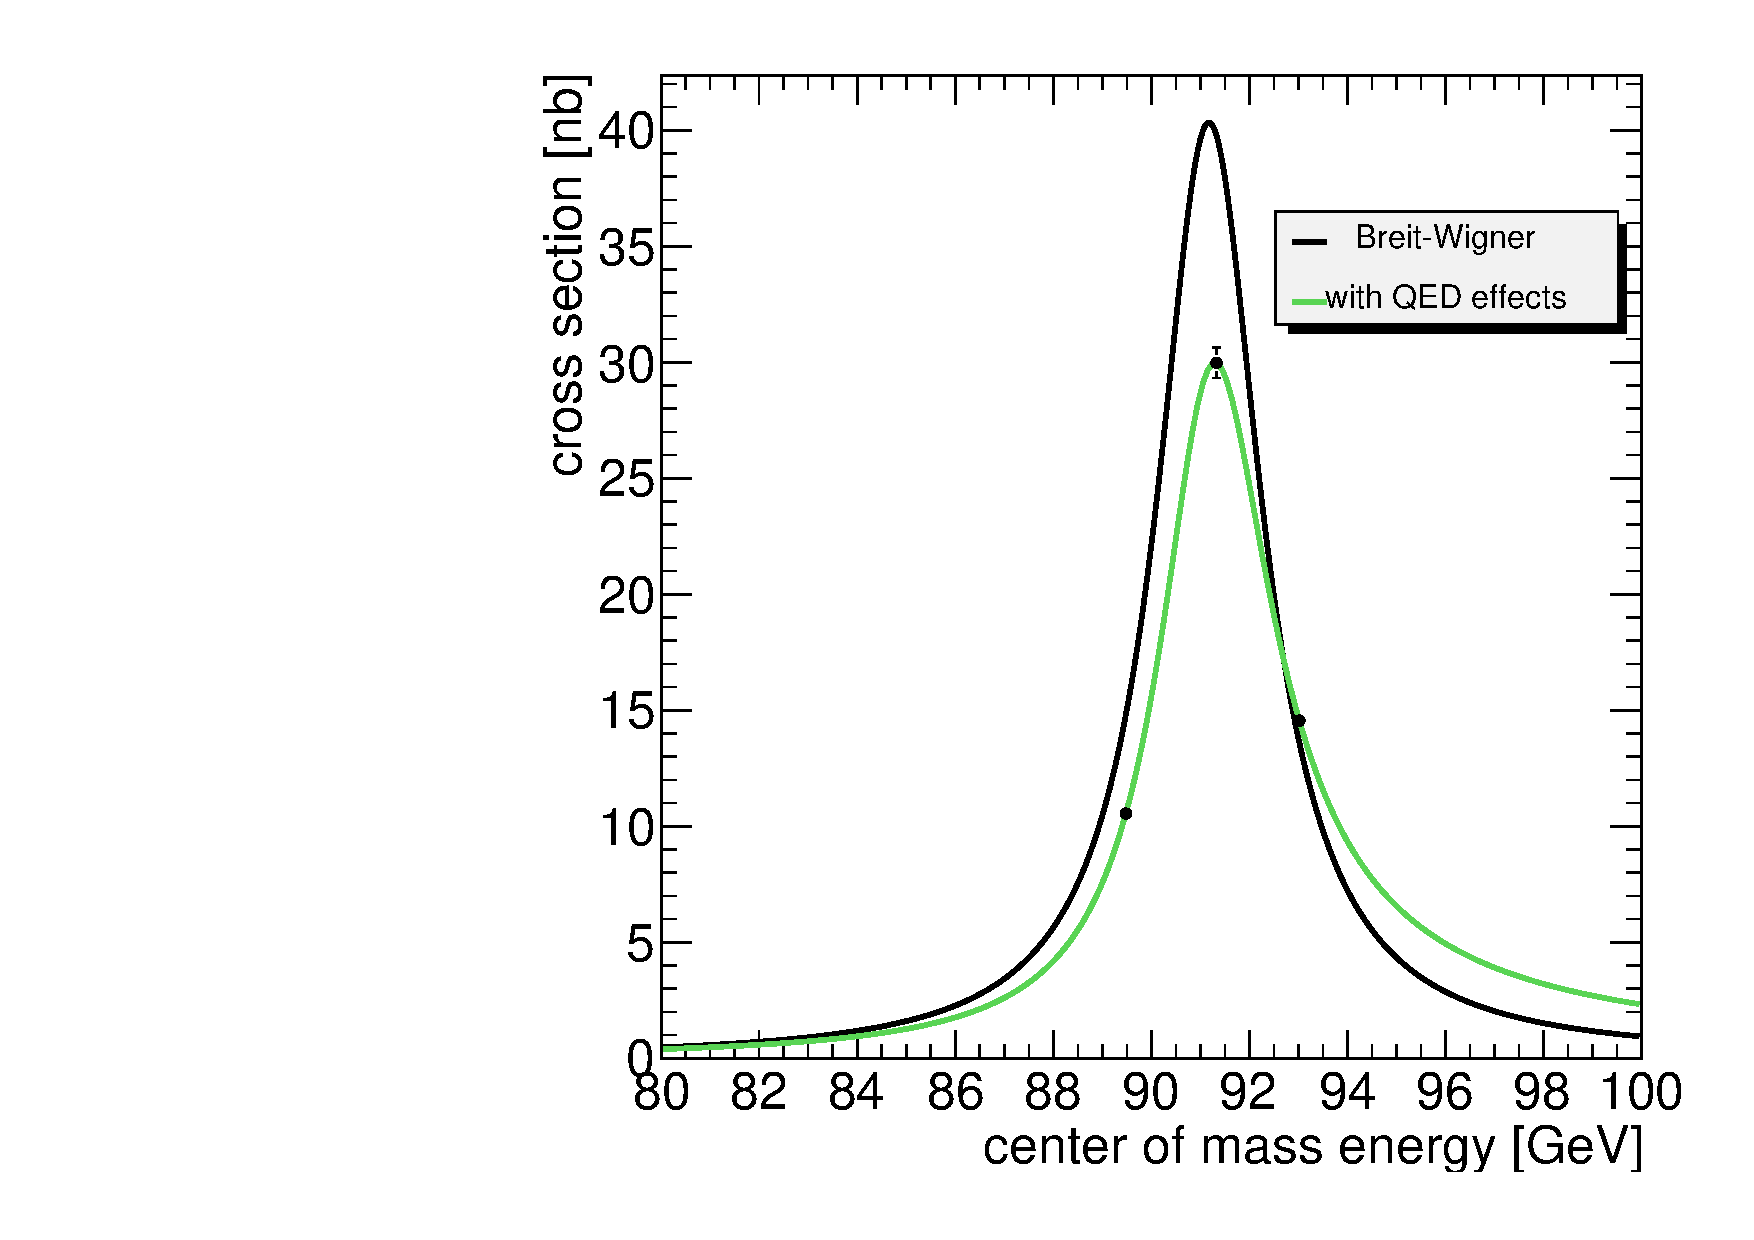
\includegraphics[width=1\columnwidth,keepaspectratio]{finalhad_fit}
 \caption{Breit-Wigner-fit for hadronic events.}
 \label{fig:fit_hadrons}
\end{figure}

\begin{table}[h]
\begin{center}
\begin{tabular}{|l|l|l|}
\hline
$M_Z$ [\si{\GeV}] & $σ_0^{\mathrm{had}}$  [\si{\nano\barn}] & $Γ_Z$
[\si{\GeV}]\\
\hline
$91.16 \pm 0.02 \pm 0.02$ & $40.33 \pm 0.65 \pm 0.27$ & $2.61 \pm 0.05 \pm 0.03$\\
\hline
\end{tabular}
\vspace*{0.3cm}
\caption{\baselineskip=0.38cm Results of fit on data. The hadronic cross section
$σ_0^{\mathrm{had}}$, the mass $M_Z$ and the decay width $Γ_Z$ of the
$Z^0$-boson is determined from the fit in \fref{fit_hadrons}.}
\label{tab:results}
\end{center}
\vspace*{-0.5cm}
\end{table}
This is the first and already very precise measurement of the mass of the $Z^0$-boson. 
% no paragraph
The χ$^2$-value of this fit is almost zero, but as there were only three points
to fit and at the same time three parameters to be evaluated, the
number of degrees of freedom (ndf) is zero. Therefore the value of $χ^2/$ndf has to be
undefined. During the next data taking periods more data at different center of
mass energies will be acquired, so that this problem will be solved.

From the decay width of the $Z^0$, it is also possible to derive the lifetime
of this particle. This is done using the following formula:
\begin{eqnarray}
τ_Z &=& \frac{1}{Γ_Z}\\
\nonumber &=& (2.53 \pm 0.31 \pm 0.02) \cdot \SI{e-25}{\second}
\end{eqnarray}

\subsection{Muonic events}

Muonic signals could be distinguished from hadronic events as well as
from background. Therefore an analysis on muonic events is possible. This is
described in this section.

Firstly, the cross sections at the different center of mass energies could be
calculated in an analogue way to the hadronic events (see \eref{sigma}). The
results of this can
be found in \tref{muon_events}.

\begin{table}[h]
\begin{center}
\begin{tabular}{|l|l|l|}
\hline
energy $\sqrt{s}$ [\si{\GeV}] & muon events & cross section $σ_0^μ$ [\si{\nano\barn}]\\
\hline
89.48 & \phantom{0}67 ± \phantom{0}8 ± \phantom{0}8  & 0.64 ± 0.03 ± 0.3 \\
91.33 & 122 ± 11 ± 10 & 1.53 ± 0.05 ± 0.4 \\
93.02 & \phantom{0}77 ± \phantom{0}9 ± \phantom{0}9 & 0.87 ± 0.04 ± 0.03 \\
\hline
\end{tabular}
\vspace*{0.3cm}
\caption{\baselineskip=0.38cm Analyzed muonic events at different center of mass
energies.}
\label{tab:muon_events}
\end{center}
\vspace*{-0.5cm}
\end{table}

Starting from these values and already knowing the decay width of the
$Z^0$-boson as well as its mass, we can again do a fit on these three data
points. The plot is shown in \fref{fit_muons}. This time the only free
parameter is the muonic cross section $σ_0^μ$, which is presented in the next
equation.
\begin{figure}[htb]
 \centering
 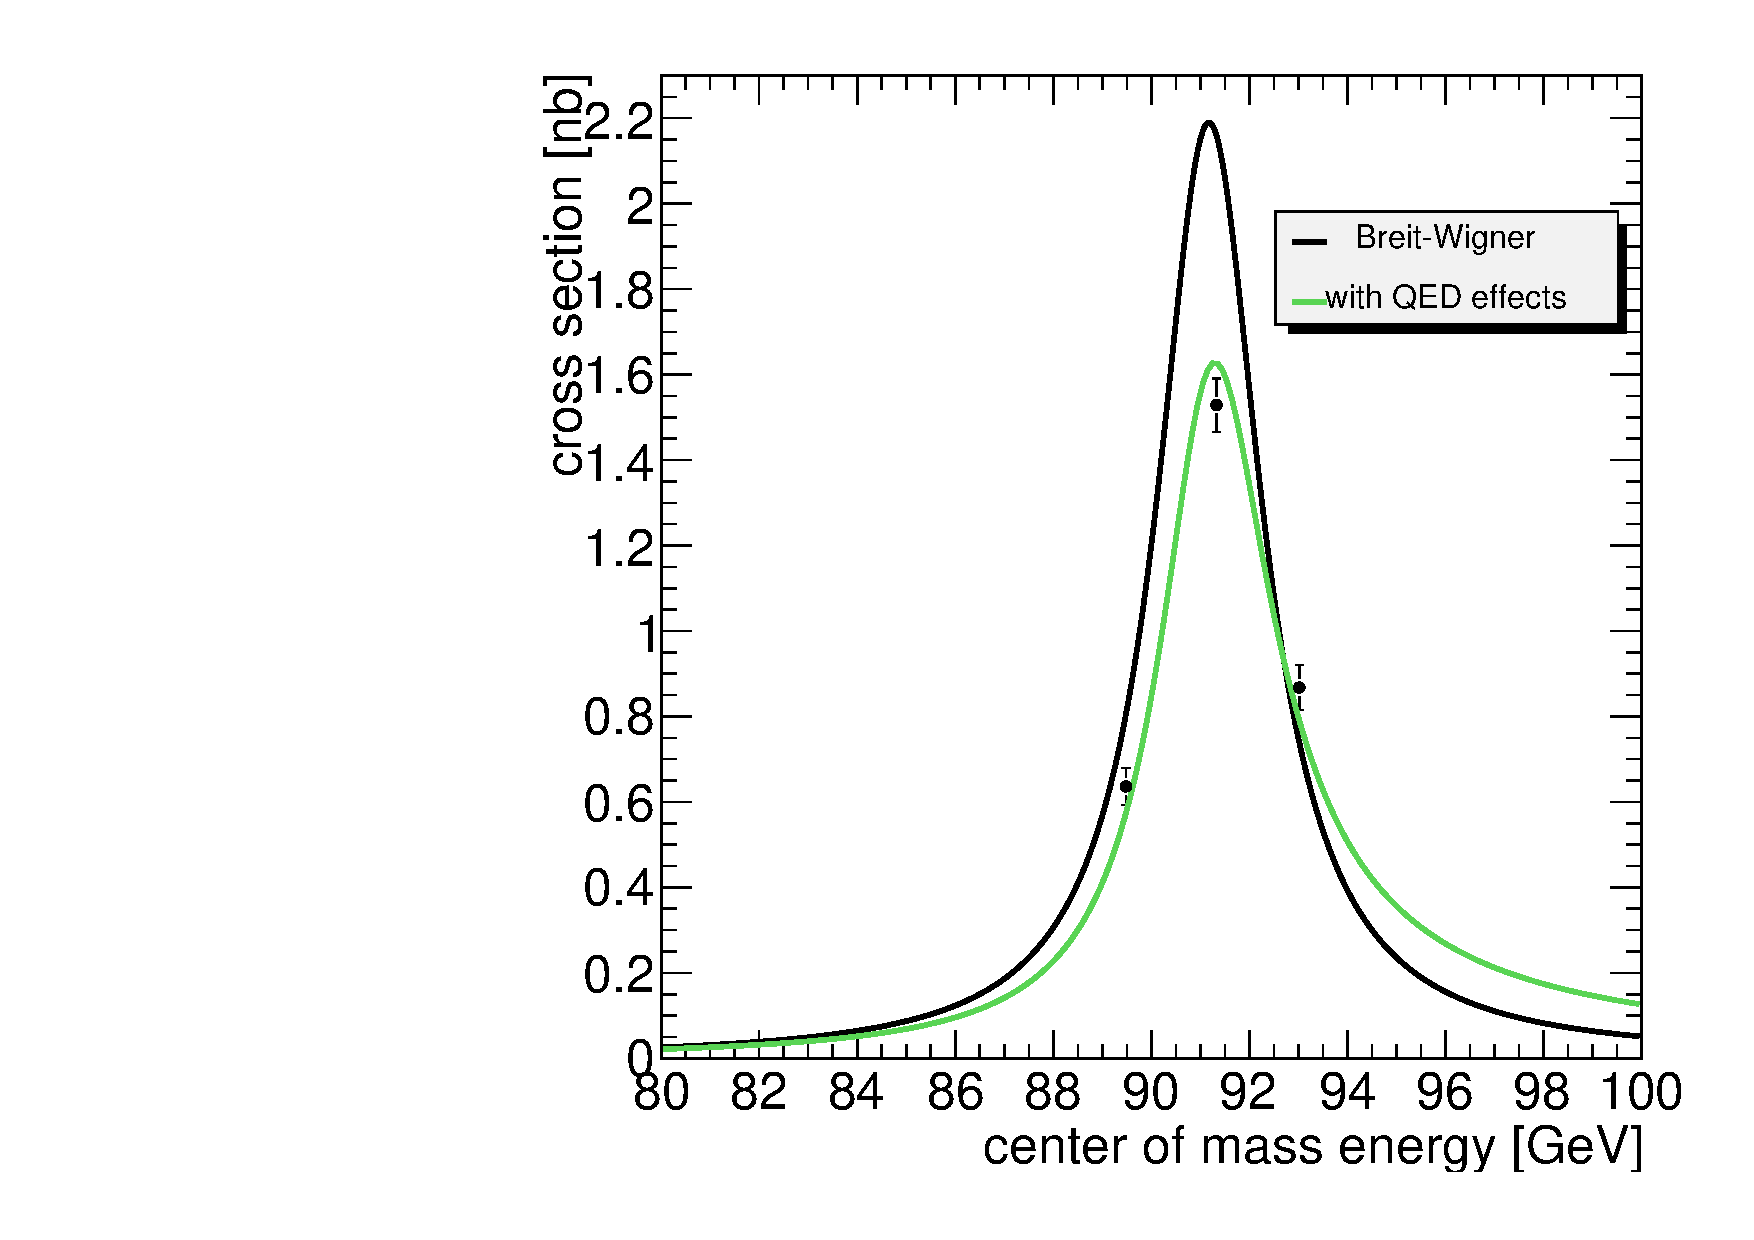
\includegraphics[width=1\columnwidth,keepaspectratio]{finalmu_fit}
 \caption{Breit-Wigner-fit for muonic events.}
 \label{fig:fit_muons}
\end{figure}
%The result of this fit is shown in the following line:
\begin{equation}
\nonumber σ_0^μ = (2.16 \pm 0.05 \pm 0.03) \si{\nano\barn}
\end{equation}
The $χ^2$-value of this fit is some 6.8, which gives a $χ^2/$ndf of about 3.4.
This is already in the right order of magnitude as it is close to a value of 1.

\subsection{Determination of the leptonic decay width}
Through the knowledge of the overall cross section it is possible to calculate
the leptonic decay width $Γ_l$. First of all we assume that the decay width is
the same for all leptons. We can use the following formula for determining it
by using the fit parameter for the muonic cross section:
\begin{equation}
σ_0^μ = \frac{12π}{M_Z^2}\frac{Γ_l^2}{Γ_Z^2}.
\label{eqn:leptonicwidth}
\end{equation}
This equation can easily be solved to determine the resulting leptonic decay
width $Γ_l$, because all the other variables are known.
\begin{equation}
Γ_l = (91 \pm 2 \pm 1)\si{\mega\electronvolt}
\label{eqn:leptonicwidthresult}
\end{equation}
In order to calculate the leptonic decay width, it is also possible to utilize
the following equation:
\begin{equation}
Γ_l = \frac{1}{3}(Γ_Z - 3Γ_{\mathrm{Had}} - 3Γ_{ν_l}).
\end{equation}
$Γ_{\mathrm{Had}}$ can be calculated in the same way as the leptonic decay
width in \eref{leptonicwidth}. $Γ_{ν_l}$ can be determined by using the
following relationship:
\begin{eqnarray}
Γ_{ν_e} &=& \frac{G_FM_Z^3}{12\sqrt{2}π}\\
&=& (165.71 \pm 0.10 \pm 0.09)\si{\mega\electronvolt}
\end{eqnarray}
Now the leptonic decay width $Γ_l$ can be evaluated.
\begin{equation}
Γ_l = (83 \pm 4 \pm 3) \si{\mega\electronvolt}
\end{equation}
This is in the same order of magnitude as the result shown in
\eref{leptonicwidthresult}. Although these two results do not agree in
one standard deviation, they do agree in two standard deviations.
Therefore it can be assumed that a more precise measurement in the future
will enable physicists to find a better agreement.

\subsection{Determination of the hadronic decay width}
\label{sec:hadrwidth}
As we now know the leptonic decay width, it is also possible to calculate the
hadronic decay width $Γ_{\mathrm{had}}$. There exists an anti-proportional relation
between these two variables, with only known constants as factors. The value for
the hadronic decay width evaluates to
\begin{equation}
Γ_{\mathrm{had}} = (1.86 \pm 0.01 \pm 0.02) \si{\giga\electronvolt}.
\end{equation}
There is also another relation which can be used to determine the value of this
decay width:
\begin{eqnarray}
Γ_{\mathrm{had}} &=& \Gamma_Z - 3\Gamma_{\nu_e} - 3\Gamma_e\\
&=& (1.86 \pm 0.05 \pm 0.03) \si{\giga\electronvolt}.
\end{eqnarray}
It is clearly visible that these two results are in perfect agreement.

\subsection{Calculation of the weak mixing angle}

The achieved results by now offer furthermore an opportunity to obtain the
weak mixing angle using the formula
\begin{eqnarray}
Γ_l &=& \frac{G_F M_Z^3}{24 \sqrt{2}π}\left(1+[1-4|Q_l|\sin² Θ_W]²\right)\,.
\end{eqnarray}
As $Γ_l$ as well as $M_Z$ is known, the expression $\sin² Θ_W$ can be computed.
\begin{eqnarray}
\sin^2\Theta_W &=& \frac{1-\sqrt{\frac{\Gamma_e\cdot 24\sqrt{2}\pi}{G_FM_Z^3}-1}}{4}\\
\label{eqn:gammaquark}
\nonumber &=& 0.23 \pm 0.05 \pm 0.08
\end{eqnarray}
Thereby the weak mixing angle is determined, too.
\begin{eqnarray}
Θ_W &=& \arcsin(\sqrt{\sin^2\Theta_W})\\
\nonumber &=& 0.50 \pm 0.11 \pm 0.07\\
\nonumber &=& (28 \pm 6 \pm 4)\symbol{23}
\end{eqnarray}
This angle is, as a parameter of the electroweak theory, a fundamental
constant describing this interaction as a symmetry group.

\subsection{Calculation of the colour factor}

Finally the measurements allow also to calculate the colour factor $N_C$ using
$Γ_{\mathrm{had}}$. The hadronic decay width was determined in \ref{sec:hadrwidth}.

In reference to the standard model there is a way to compute $N_C$.
\begin{equation}
 Γ_{\mathrm{had}} = N_C \cdot K_{QCD}\cdot ( 2Γ_u + 3Γ_d )
 \label{eqn:gammahad2}
\end{equation}
The decay widths $Γ_u$ and $Γ_d$ can be calculated by the standard model, using the
value of the Weinberg angle as seen in \eref{gammaquark}. The charges of the up-quark was
set to $\frac{2}{3}$ and the charge of the down-quark to $-\frac{1}{3}$. Then the colour
factor can be calculated.
\begin{equation}
 N_C = 3.20 \pm 0.11 \pm 0.07
\end{equation}
This result confirms, that there are no new quarks to be expected with a mass
lower than some \SI{45}{\GeV}.


% \begin{table}[h]
% \begin{center}
% \begin{tabular}{|l|l|l|}
% \hline
% \multicolumn{1}{|c|}{}& proton & deuteron\\
% \hline
% \multicolumn{3}{|c|}{Exclusive electroproduction}\\
% \hline
% $A^\rho_1$       & 0.23 $\pm$ 0.13$\pm$0.01 & -0.040 $\pm$ 0.076$\pm$0.003\\ 
% $A^\phi_1$       & 0.20$\pm$0.45$\pm$0.01  & 0.17$\pm$0.27$\pm$0.01\\
% $N^\rho$         &1774                   & 6505\\
% $N^\phi$         & 219                   & 618 \\
% \hline
% \multicolumn{3}{|c|}{Electroproduction by quasi-real photons}\\
% \hline
% $A^\rho_1$  & 0.0057 $\pm$ 0.0093$\pm$0.0004  & -0.0039 $\pm$
% 0.0029$\pm$0.0003\\ 
% $A^\phi_1$  & 0.052 $\pm$ 0.084$\pm$0.003  & 0.018 $\pm$ 0.028$\pm$0.001\\
% $N^\rho$    & $423\times10^{3}$ & $4013\times10^{3}$\\
% $N^\phi$ & $7.6\times10^{3}$ &  $57\times10^{3}$ \\
% \hline
% \end{tabular}
% \vspace*{0.3cm}
% \caption{\baselineskip=0.38cm Example of a table}
% \label{tab_asy}
% \end{center}
% \vspace*{-0.5cm}
% \end{table}


\section{ Summary}
In order to sum up the results one has to say that this is a first
confirmation of the predictions of the standard model. The properties of the
predicted $Z^0$-boson could be measured precisely. Additionally the first exact
measurement of the weak mixing angle was done successfully, which was one of the
most important tasks of this experiment.

It has to be mentioned that the background was found to be negligible and
therefore it was not included in the calculations. This could be done in a
further study. During the next months of data taking, there will also be higher
luminosities available as well as measurements at higher center of mass
energies, which will improve the resuls of this study.

\begin{thebibliography}{}
\baselineskip=0.38cm
\bibitem{pic} http://ams.pg.infn.it/ams-italy/pub/5\_5.htm
\bibitem{tdr} CERN (1984). "LEP design report". Geneva.
\bibitem{pdb} C. Amsler et al. (2008). "Review of Particle Physics". Physics Letters B 667

\end{thebibliography}
% 
% \listoftodos

% \begin{figure}[htb]
%  \centering
%  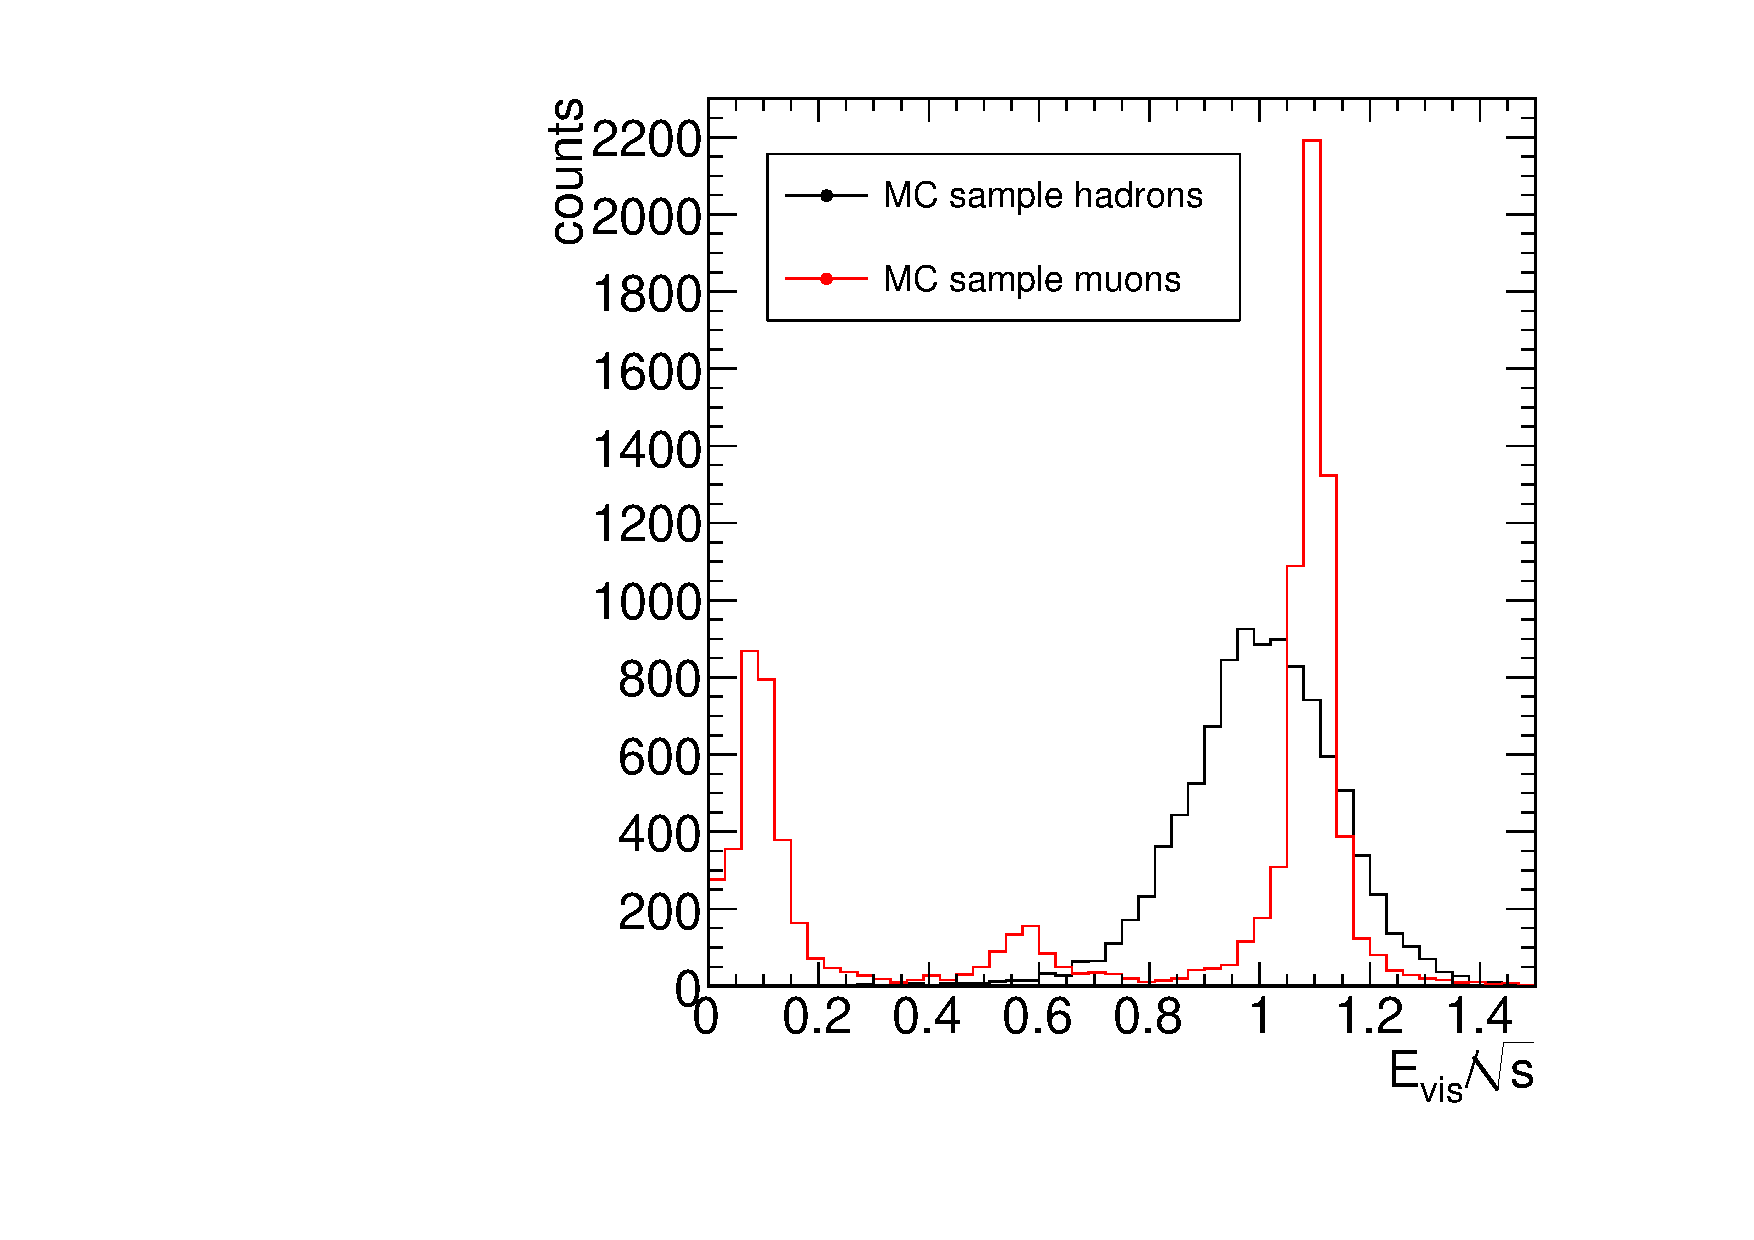
\includegraphics[width=1\columnwidth,keepaspectratio]{E_vis}
%  \caption{Distribution of visible energie}
%  \label{fig:e_vis}
% \end{figure}
% 
% \begin{figure}[htb]
%  \centering
%  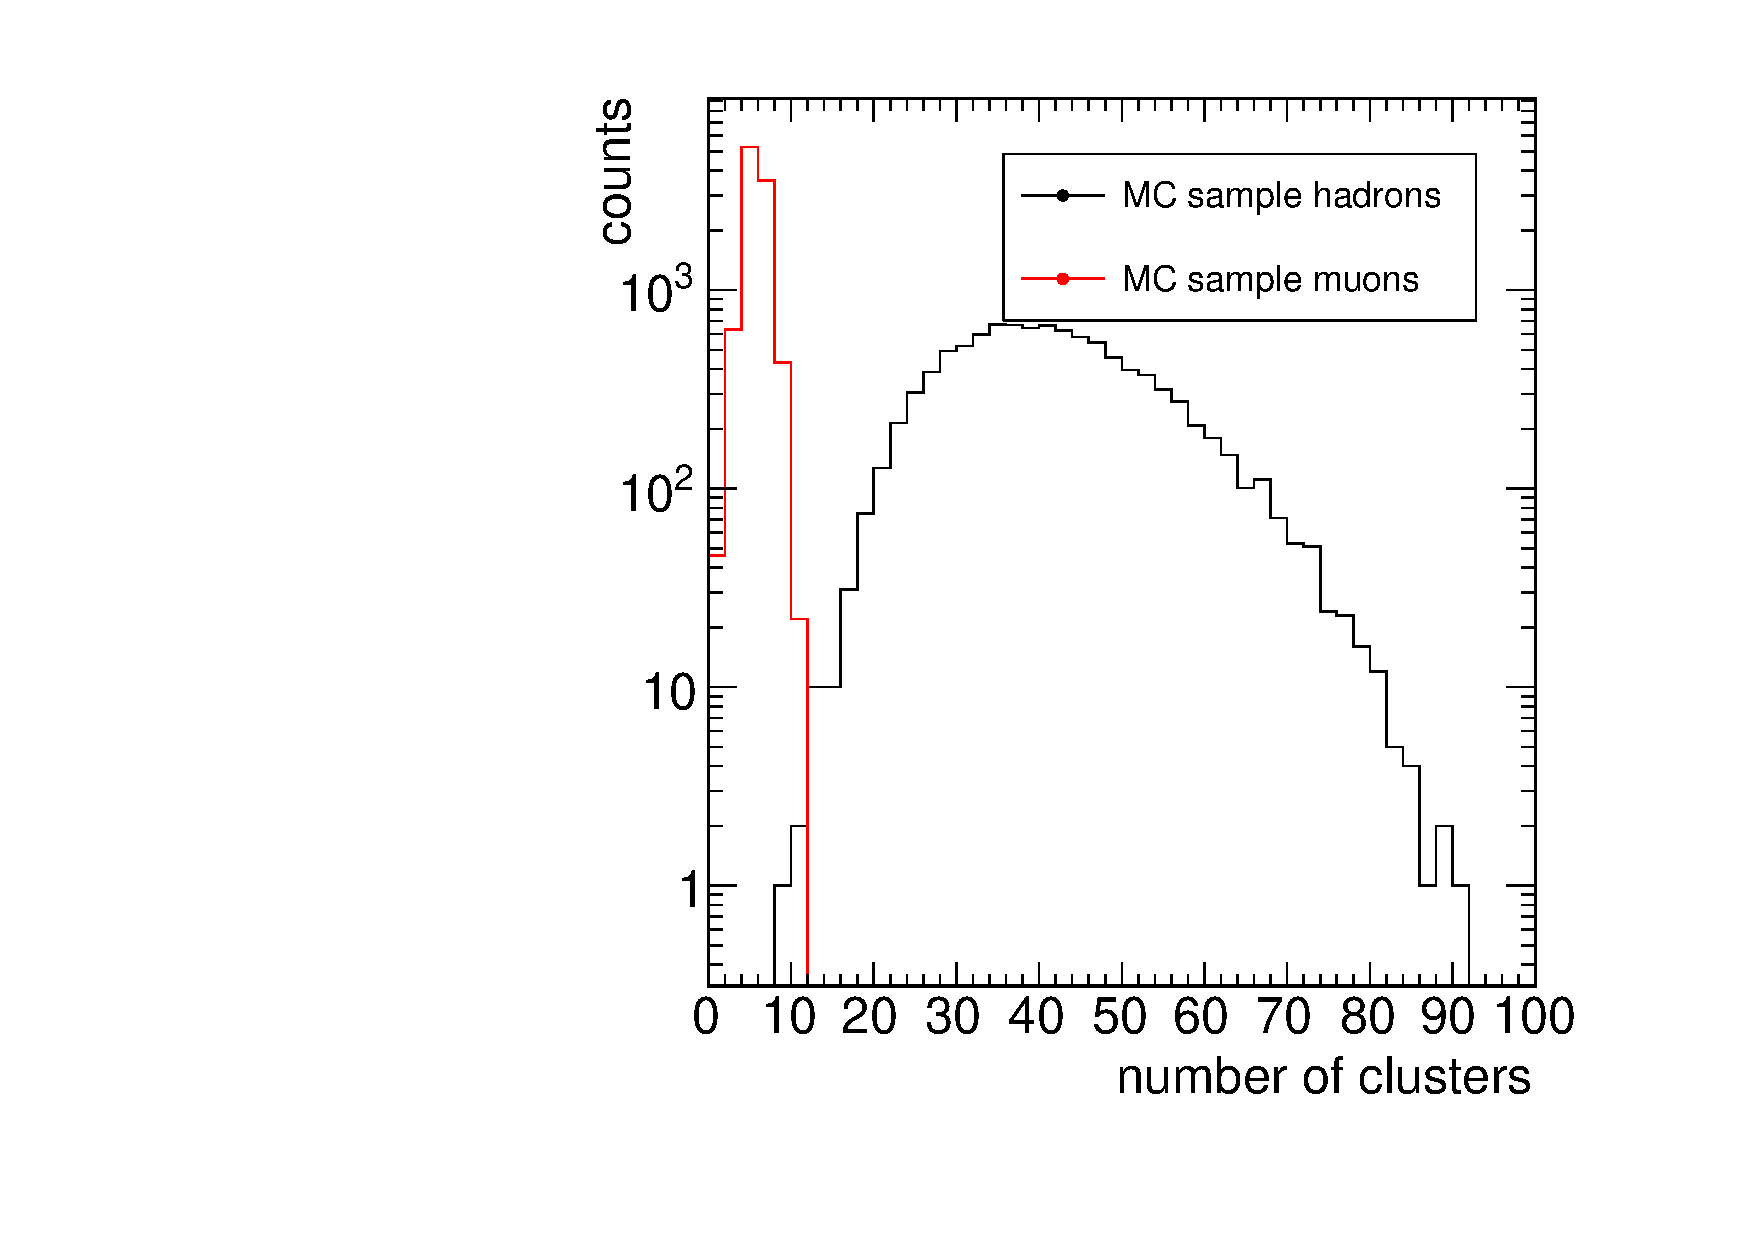
\includegraphics[width=1\columnwidth,keepaspectratio]{N_Cluster}
%  \caption{Distribution of entries in the calorimetre}
%  \label{fig:n_cluster}
% \end{figure}

\end{document}
